%%
%% This is file `sample-sigconf.tex',
%% generated with the docstrip utility.
%%
%% The original source files were:
%%
%% samples.dtx  (with options: `all,proceedings,bibtex,sigconf')
%%
%% IMPORTANT NOTICE:
%%
%% For the copyright see the source file.
%%
%% Any modified versions of this file must be renamed
%% with new filenames distinct from sample-sigconf.tex.
%%
%% For distribution of the original source see the terms
%% for copying and modification in the file samples.dtx.
%%
%% This generated file may be distributed as long as the
%% original source files, as listed above, are part of the
%% same distribution. (The sources need not necessarily be
%% in the same archive or directory.)
%%
%%
%% Commands for TeXCount
%TC:macro~\cite [option:text,text]
%TC:macro~\citep [option:text,text]
%TC:macro~\citet [option:text,text]
%TC:envir table 0 1
%TC:envir table* 0 1
%TC:envir tabular [ignore] word
%TC:envir displaymath 0 word
%TC:envir math 0 word
%TC:envir comment 0 0
%%
%% The first command in your LaTeX source must be the \documentclass
%% command.
%%
%% For submission and review of your manuscript please change the
%% command to \documentclass[manuscript, screen, review]{acmart}.

\documentclass[sigconf]{acmart}
%%
%% \BibTeX command to typeset BibTeX logo in the docs
\AtBeginDocument{%
  \providecommand\BibTeX{{%
    Bib\TeX}}}

\setcopyright{acmlicensed}
\copyrightyear{2018}
\acmYear{2018}
\acmDOI{XXXXXXX.XXXXXXX}
\acmConference[Conference acronym 'XX]{Make sure to enter the correct
  conference title from your rights confirmation emai}{June 03--05,
  2018}{Woodstock, NY}
\acmISBN{978-1-4503-XXXX-X/18/06}

\usepackage[ruled,vlined]{algorithm2e}
\SetKwInput{KwGlobalIn}{Global Mem Input}
\SetKwInput{KwSharedIn}{Shared Mem Input}
\SetKwInput{KwSharedOut}{Shared Mem Output}
\SetKwInput{KwGlobalOut}{Global Mem Output}
\SetKwInput{KwConstants}{Constants}

\usepackage{amsmath}
\usepackage{mathtools}
\usepackage{listings}
\usepackage{subcaption}
\newcommand{\thomas}[1]{{\footnotesize\color{orange}[Thomas: #1]}}
\newcommand{\john}[1]{{\footnotesize\color{cyan}[John: #1]}}
\newcommand{\raph}[1]{{\footnotesize\color{magenta}[Raph: #1]}}

\begin{document}

\title{The Name of the Title Is Hope}

\author{Lars Th{\o}rv{\"a}ld}
\affiliation{%
\institution{The Th{\o}rv{\"a}ld Group}
\city{Hekla}
\country{Iceland}}
\email{larst@affiliation.org}

\author{Valerie B\'eranger}
\affiliation{%
  \institution{Inria Paris-Rocquencourt}
  \city{Rocquencourt}
  \country{France}
}

\author{Aparna Patel}
\affiliation{%
  \institution{Rajiv Gandhi University}
  \city{Doimukh}
  \state{Arunachal Pradesh}
  \country{India}}

\renewcommand{\shortauthors}{Trovato et al.}

\begin{abstract}
  TODO
\end{abstract}

\begin{CCSXML}
  <ccs2012>
  <concept>
  <concept_id>00000000.0000000.0000000</concept_id>
  <concept_desc>Do Not Use This Code, Generate the Correct Terms for Your Paper</concept_desc>
  <concept_significance>500</concept_significance>
  </concept>
  <concept>
  <concept_id>00000000.00000000.00000000</concept_id>
  <concept_desc>Do Not Use This Code, Generate the Correct Terms for Your Paper</concept_desc>
  <concept_significance>300</concept_significance>
  </concept>
  <concept>
  <concept_id>00000000.00000000.00000000</concept_id>
  <concept_desc>Do Not Use This Code, Generate the Correct Terms for Your Paper</concept_desc>
  <concept_significance>100</concept_significance>
  </concept>
  <concept>
  <concept_id>00000000.00000000.00000000</concept_id>
  <concept_desc>Do Not Use This Code, Generate the Correct Terms for Your Paper</concept_desc>
  <concept_significance>100</concept_significance>
  </concept>
  </ccs2012>
\end{CCSXML}

\ccsdesc[500]{Do Not Use This Code~Generate the Correct Terms for Your Paper}
\ccsdesc[300]{Do Not Use This Code~Generate the Correct Terms for Your Paper}
\ccsdesc{Do Not Use This Code~Generate the Correct Terms for Your Paper}
\ccsdesc[100]{Do Not Use This Code~Generate the Correct Terms for Your Paper}

\keywords{Do, Not, Us, This, Code, Put, the, Correct, Terms, for,
  Your, Paper}

\received{20 February 2007}
\received[revised]{12 March 2009}
\received[accepted]{5 June 2009}

\maketitle

\section{Introduction (WIP)}
 (Tell readers we are targeting WebGPU)
 (Speed of light definition here)
\subsection{Goals of a Scan Implementation}
\begin{itemize}
  \item \textbf{Minimal global memory access:} the scan should minimize global memory access to the theoretical minimum of $2n$.
  \item \textbf{Fully saturates global memory bandwidth:} the scan should be capable of fully saturating the global memory bandwidth.
  \item \textbf{Portability:} the scan should be portable across hardware vendors and architectures.
\end{itemize}
\thomas{See comment in section 3 !}
Our method retains the best aspects of the \emph{Chained-Scan} architecture, while eliminating the need for forward progress guarantees. It is designed to operate on arbitrary hardware, support arbitrary monoids, process inputs of arbitrary size, and support arbitrary 32-bit and 64-bit data types.
\subsection{Goals}
This work is guided by two main goals:
\begin{enumerate}
  \item \textbf{Portability}: we want to develop a scan implementation that retains the benefits of the \emph{Chained-Scan} architecture but is also suitable for a diverse range of hardware vendors and architectures, including those without FPG or support for 64-bit atomics.
  \item \textbf{Performance}: we aim for near speed-of-light execution to the greatest extent possible allowed by the underlying hardware and programming model.
\end{enumerate}

\noindent
To ground these objectives, we select the WebGPU shading language (WGSL) and the WebGPU standard as our target environment. WGSL is a meta-level shading language which is translated and compiled as necessary for backend graphics APIs---D3D12, Vulkan, and Metal---and as such, WGSL implementations are bound by the minimum capability across all backends. Because WGSL must operate within this limited capability space, it inherently embodies the challenge of portability.

\subsection{Non Goals}
Although our goal is to create a fully portable and highly performant scan implementation, we are constrained by underlying hardware platforms and programming models. As discussed in more detail in \emph{Limits on the Speed-of-Light}, not all architectures offer atomic operations that are sufficiently fast enough or scheduling models that are sufficiently fair enough to attain speed-of-light performance, and thus we cannot guarantee such performance. Although we are cognizant of the risks posed by subgroup divergence, subgroup functions in shading languages do not allow explicit divergence control,\footnote{For example, CUDA allows developers to explicitly provision subgroup functions with a mask of the threads that will participate in them.} placing a solution to subgroup divergence issues outside our scope. Lastly, we do not investigate alternative $O(2n)$ scan architectures beyond \emph{Chained-Scan}.

\subsection{Contributions}
\begin{enumerate}
  \item Decoupled-Fallback
  \item Split-Method
  \item Subgroup-Size Agnostic stuff
\end{enumerate}

\section{Background}
\subsection{Virtualization and Scheduling in the GPU programming model}
Contemporary GPUs are hierarchically organized, massively parallel processors designed to prioritize throughput over latency. (one sentence on thread hierarchy maybe). As comprehensive descriptions of the GPU programming model~\cite{} already exist, we focus on the aspects most relevant to this work: scheduling and synchronization.

On GPU hardware, scheduling is divided into two levels: a \emph{workgroup} scheduler, which manages kernel launches and maps virtual processors, workgroups, to physical processors, \emph{multiprocessors}, and a \emph{subgroup} scheduler, responsible for selecting which of the currently \emph{occupant} subgroups on a multiprocessor for execution. The GPU programming model virtualizes processors to ensure GPU programs---\emph{kernels}---remain portable across hardware with differing physical resources. Effective virtualization requires \emph{oversubcription}, a programming paradigm where tasks are (over)partitioned in such a way that kernels request more virtual processors than are physically available. As a result, a single multiprocessor may host multiple workgroups simultaneously. However, as a consequence of virtualization, the developer relinquishes control over the order in which workgroups are launched, and once a workgroup begins execution on a multiprocessor, it must run to completion and cannot context switch.

\subsubsection{Inter-Workgroup Barriers}
Although threads \emph{within} a workgroup may synchronize with each other by participating in a \emph{barrier} primitive, the virtualization of processors introduces an emergent high-level limitation: the absence of an inter-workgroup barrier. As previously mentioned, workgroups cannot context switch. Although contemporary GPU hardware~\cite{} supports workgroup preemption for prioritizing real-time tasks or managing multi-process workloads, this functionality is deliberately excluded from the GPU programming model. This stems from the prohibitively high overhead in latency and storage associated with moving workgroup contexts on and off chip. In the oversubscription paradigm, where the number of workgroups is theoretically unbound and typically far exceeds the available multiprocessors, every invocation of such a barrier would necessitate context-switching between all launched workgroups. Due to this high cost, no GPU programming environment furnishes developers with a true unbounded-launch inter-workgroup barrier.\footnote{CUDA recently introduced \emph{Thread Block Cluster} synchronization~\cite{NvidiaCudaGuide}, but it is almost certainly designed to operate within the \emph{Persistent-Thread}~\cite{gupta2012} paradigm, rather than serving as a barrier across an unbounded launch.} Instead, when inter-workgroup synchronization is necessary, developers must rely on kernel launches as synchronization points. However, kernel launches are suboptimal as barriers: they incur overheads due to the heterogeneous nature of the operation, and all execution context is lost between launches.

\subsubsection{Fairness and Progress}
Because multiple workgroups may reside on a single multiprocessor, two key issues arise at the subgroup scheduling level: \emph{fairness}---how evenly execution resources are distributed among threads---and \emph{progress guarantees}---ensuring that all threads or subgroups eventually make progress towards termination. However, the term "fairness" is used differently across the literature, leading to potential confusion. Sorensen et al.\cite{sorensen2016,sorensen2018,sorensen2021}, whose work provides the most comprehensive taxonomy of progress models to date, use "fairness" specifically to describe differing levels of progress guarantees. In contrast, NVIDIA publications~\cite{4523358,Merrill2016} define "fairness" in terms of the distribution of execution resources among subgroups. In this work, we adopt NVIDIA's terminology to maintain consistency with their publications, while acknowledging the broader definitions provided by Sorensen et al.

\thomas{A scheduler may be fair but may not have FPG (M1 Pro for example); a scheduler may have FPG but may not be fair (ARM Mali). \newline
  Sorensen calls FPG "fairness:" "We have described two schedulers: fair and unfair, under which starvation-freedom for blocking idioms is either always or never guaranteed."\newline
  Nvidia, by contrast uses fairness in line with our language. From Tesla architecture: \newline
  "A scoreboard qualifies each warp for issue each cycle. The instruction scheduler prioritizes all ready warps and selects the one with highest priority for issue. Prioritization considers warp type, instruction type, and 'fairness' to all warps executing in the SM\@." \newline
  From DecoupledLookback: \newline
  "Safety. The algorithm will run to completion if the system guarantees forward-progress for all processors." \newline
  "Blocking will be minimal for systems that provide fair or nearly-fair scheduling. Fairness ensures that all processors will have recorded their aggregates in roughly the same amount of time."
}

\subsection{The Scan Primitive}\label{sec:the-scan-primitive}
The study of \emph{scan} (\emph{parallel prefix}) networks traces back to the design of carry-lookahead adder circuits and beyond~\cite{5219801,10.5555/1098666}. A scan is typically defined on a monoid \( M \), characterized by a binary reduction operator \( \oplus \) and an identity element \( \varepsilon \). The binary operator \( \oplus \) satisfies the closure property \( \forall a, b \in M, \ (a \oplus b) \in M \) and has an identity element \( \exists \varepsilon \in M, \ \forall a \in M, \ \varepsilon \oplus a = a \). Although \( \oplus \) must be associative, it is not necessarily commutative, as demonstrated in structures like the \emph{bicyclic semigroup}~\cite{}\footnote{Despite its name, this is a monoid.} and Rabin-Karp's \emph{second fingerprinting method for string matching}~\cite[Section 6]{Karp:1987:ERP}. In a scan, the result at the \( n \)-th element is the reduction of the preceding subset of elements in the sequence. If the subset includes the \( n \)-th element, it is called \emph{inclusive}; if it excludes the \( n \)-th element, it is called \emph{exclusive}. The most common scan type is the prefix sum, where \( \oplus \) is addition. For example:
\[
  x = [x_1, x_2, x_3, \dots, x_n] \ \ \ \ \ \ \ y = [1, 1, 1, 1, 1]
\]
\[
  \text{InclusiveScan}(x, \oplus) = [x_1, x_1 \oplus x_2, x_1 \oplus x_2 \oplus x_3, \dots, x_1 \oplus x_2 \oplus \cdots \oplus x_n]
\]
\[
  \text{InclusiveScan}(y, +) = [1, 2, 3, 4, 5]
\]
Due to its significance in circuits and as a fundamental algorithmic primitive, scan has been extensively studied in both electrical engineering and computer science. Harris~\cite{1292373} offers a taxonomy that relates depth, fanout, and wire tracks, while Hinze~\cite{10.1007/978-3-540-27764-4_11} develops an algebraic framework for scans. Snir~\cite{10.1016/0196-67748690003-9} proved that depth $d$ and size $s$ are related by $s + d \ge 2n - 2$, and Fich~\cite{10.1145/800061.808738} proved that among minimum depth scans Ladner-Fischer~\cite{10.1145/322217.322232} networks have optimal size. Blelloch~\cite{} adapted scan to the PRAM model and popularized its use as an algorithmic primitive. Finally, Merrill and Garland~\cite{Merrill2016} provide a review of GPU scan implementations, complementing earlier work by Merrill and Grimshaw~\cite{Merrill2009}.

\subsection{Evolution of Inter-Workgroup Scan Architectures}
Contemporary GPU scans are distinguished from earlier PRAM-like scans~\cite{} by their alignment with the GPU memory hierarchy, which grades memory into progressively faster but increasingly private tiers. To operate efficiently, GPU scans must hybridize fine-grain intra-workgroup (\emph{local}) strategies, executed privately within shared memory and registers, with coarse-grain inter-workgroup (\emph{global}) strategies, performed in global memory. Due to their relatively low arithmetic intensity, it is theoretically expected and experimentally observed that the performance of local scans are memory-bound, as first demonstrated by Merrill and Grimshaw~\cite{}. Consequently, once equipped with a sufficient local scan strategy, the focus of scan design shifts to addressing the challenges of the global strategy, particularly inter-workgroup coordination and synchronization. In this section, we review the three prominent GPU global scan strategies---\emph{Scan-then-Propagate}, \emph{Reduce-then-Scan}, and \emph{Chained-Scan}---examining how they navigate inter-workgroup dependencies and evaluating their effectiveness in minimizing global memory access and maximizing memory bandwidth utilization.

\subsubsection{Scan-then-Propagate}
Introduced by Sengupta et al.~\cite{10.5555/1280094.1280110}, the \emph{Scan-then-Propagate}~\cite{GPUGems3, Sengupta2011} strategy is an intuitive extension of the intra-workgroup scan, comprising three phases:
\begin{enumerate}
  \item \textbf{Intra-Workgroup (Local) Scan:} Each workgroup performs an inclusive scan on its assigned work tile partition of the input data. The results, including both the local scan output and the reduction of each workgroup, are written back to global memory.
  \item \textbf{Spine Scan:} The reductions from all workgroups, collectively referred to as \emph{spine}, are gathered and scanned to compute the global prefix of the reductions, resolving the dependencies between work tiles; we call the result of this phase the \emph{root}. For large scans, this stage is an insignificant amount of work compared to the first and third.
  \item \textbf{Propagation:} Each workgroup retrieves its portion of the root and combines it with the result of the local scan to compute the final scan.
\end{enumerate}

As each work tile depends on the reductions of previous tiles, the absence of an inter-workgroup barrier necessitates kernel launches to resolve inter-workgroup dependencies. This results in the three-phase construction of \emph{Scan-then-Propagate}, with each phase implemented as a separate kernel launch. This is further complicated in Sengupta et al.'s implementation, where arbitrarily large inputs are processed through recursion. As the size of a work tile limits the maximum number of elements processed without inter-workgroup dependency resolution, the three-phase scan structure must be recursively applied until the spine size fits within a single work tile. Thus, an input of size $n$ and a work tile of size $t$ results in a recursive depth of $\lceil \log_t n \rceil$, and $2\cdot\lceil \log_t n \rceil - 1$ kernel launches. Each recursive step $k$ processes $n/t^k$ tiles, leading to a total of $\sum_{k=1}^{\lceil \log_t n \rceil} n/t^k \approx (n - 1)/(t - 1)$ work tiles over all steps. Since each tile moves $4t$ data ($2t$ local scan, $2t$ propagation), the total global data movement is $O\left(\frac{4t(n - 1)}{t - 1}\right) = O(4n)$.

\subsubsection{Reduce-then-Scan}
If memory bandwidth resources are sufficiently scarce relative to compute, memory-bound algorithms like scan can profit by trading additional computation for reduced memory traffic. This trade-off led to a refinement of the \emph{Scan-Then-Propagate} strategy called \emph{Reduce-Then-Scan}~\cite{10.1145/1375527.1375559, Merrill2009, 10.1109/TPDS.2012.336, 10.5555/2031978.2032029}: by writing only the work tile reduction to global memory in the first phase and performing a redundant scan in the third phase, $n$ global data movement can be eliminated. Like \emph{Scan-then-Propagate}, \emph{Reduce-then-Scan} employs a three-phase approach using kernel launches to resolve dependencies.
\begin{enumerate}
  \item \textbf{Work Tile Reduction:} Each workgroup performs a pure reduction on its work tile partition, posting the result to global memory.
  \item \textbf{Spine Scan:} The spine is gathered and scanned to produce the root.
  \item \textbf{Intra-Workgroup Scan and Propagation:} Each workgroup performs the local scan on the work tile, incorporating its portion of the root as it writes to global memory.
\end{enumerate}

Merill and Grimshaw~\cite{Merrill2009} introduced a workgroup \emph{raking} technique that elides the overhead incurred when the recursive depth exceeds two. In this approach, the total workgroup occupancy $o$ is determined, and the input is partitioned into non overlapping blocks of size $\frac{n}{t \cdot o}$, which are raked serially by each workgroup. This limits the size of the spine from variably sized, proportional to the input size (possibly requiring recursion), to constant sized, and guaranteed to avoid further recursion. Assuming $t \geq o$, global memory movement during the spine scan is reduced from $O(n/t)$ to $O(2o)$. Kernel launches are limited to three and total global memory movement is reduced to $O(3n + 4o) = O(3n)$.

Breitbart~\cite{10.5555/2031978.2032029} was the first to apply more advanced inter-workgroup synchronization techniques to scan. Recognizing that workgroup raking naturally aligns with a \emph{Persistent-Threads}~\cite{gupta2012} paradigm, Breitbart utilized an atomics-based inter-workgroup barrier to replace kernel launches. Since multiprocessors are not oversubscribed in raking, workgroups remain resident (persist) on the multiprocessors for the entire lifetime of the kernel, enabling synchronization at the barrier without requiring context switching. Although global data movement remains at $O(3n)$, this consolidates the scan to a single kernel, minimizing launch overheads. \thomas{This also requires FPG, but not ideal to unpack and mention here . . .}

\subsubsection{Chained-Scan, Stream-Scan}
First introduced by Yan et al.~\cite{10.1145/2442516.2442539} in \emph{Stream-Scan}, the key innovation of the \emph{Chained-Scan} architecture lies in its hybridization of parallel and serial strategies: achieving parallelism at the intra-workgroup level while minimizing global data movement through serial scan operations at the inter-workgroup level. Instead of using kernel launches as inter-workgroup synchronization points, \emph{Chained-Scans} launch a single kernel that assigns work tiles in a serial order to workgroups, utilizing atomics and bit-packed status flags to ensure coherent views of data. To enforce this serial ordering, work tiles are dynamically assigned using atomic increment operations, rather than arbitrary assignment based on virtualized workgroup indices. This shifts dependency resolution from explicit synchronization via barrier-like structures to implicit synchronization via access order. As a result, each element is read and written exactly once, achieving the theoretical minimum of $2n$.

In any \emph{Chained-Scan}, once a workgroup computes its local reduction, it must complete two objectives: communicate its reduction to successor tiles and incorporate the reductions of all preceding tiles. In \emph{StreamScan}, this is facilitated by a \emph{propagation} phase, where each workgroup waits for its immediate predecessor to complete, ingests the predecessor's reduction, and posts the resulting \emph{inclusive} reduction for its immediate successor to consume. During this waiting period, the workgroup is continually scheduled, and the \emph{progress} of other workgroups must be guaranteed to prevent the spinning workgroup from starving its dependent predecessors of execution, which could result in deadlock.

While \emph{StreamScan} successfully reduces per-element device memory accesses to two, it does not consistently saturate global memory bandwidth, preventing it from achieving speed-of-light performance. This limitation arises because a workgroup in \emph{StreamScan} cannot post its reduction to global memory until it has received the result of its immediate predecessor. While this results in efficient $O(n/t)$ communication of reductions, and $O(2n+ n/t)= O(2n)$ total data movement, the sequential dependency creates a bottleneck that limits performance to the rate at which reductions propagate through device memory. Although this can be mitigated by increasing the size of the work tile, limited on-chip resources preclude scaling the tile size indefinitely. Moreover, this approach is unsuitable for a portable environment, as excessively large work tiles risk reducing occupancy on less capable hardware.

\subsubsection{Chained-Scan, Decoupled-Lookback}
Merrill and Garland~\cite{Merrill2016} introduced the \emph{Decoupled-Lookback} technique, which separates reduction propagation and dependency resolution to address the bottleneck caused by propagation latency. In this approach, each workgroup posts its local reduction to global memory and then performs a \emph{lookback}---a serial traversal backward along the spine---to compute its inclusive reduction. Work and memory accesses are constant-bounded to the workgroup occupancy $o$ by posting the inclusive reduction after the lookback. However, granting each workgroup control over its dependency resolution does not eliminate reliance on \emph{progress guarantees}, as workgroups must still spin on tiles that have yet to post their reductions, risking deadlock.

Although \emph{Decoupled-Lookback} increases global memory access during the propagation phase to $O(o(n/t))$, the serial ordering of work tile processing confines spine memory accesses to a roughly $o$-width sliding window, making them highly likely to be cache-resident. As a result, the additional global memory traffic along the spine introduces a negligible latency overhead. With total global memory movement of $O(2n+o(n/t))= O(2n)$, \emph{Decoupled-Lookback} achieves full utilization of device memory bandwidth and delivers speed-of-light performance without the work tile size tuning required by \emph{Stream-Scan}.

\subsection{Ideal Scan Architecture}
The design of an ideal scan architecture must balance performance, portability, and practicality. Beyond their differences in speed, \emph{Chained-Scan} and \emph{Reduce-Then-Scan} embody two fundamentally contrasting paradigms. By eliding explicit inter-workgroup synchronization, \emph{Chained-Scan} aligns naturally with the oversubscription paradigm, delegating occupancy management to the hardware scheduler. In contrast, the raking approach inherent to \emph{Reduce-Then-Scan} mandates the fixed-launch paradigm, necessitating explicit control over occupancy and potentially synchronization.

Fixed-launch approaches demand substantial developer effort, requiring either tuning of workgroup launch sizes across target devices or occupancy discovery. Moreover, previous workgroup occupancy discovery techniques, such as the one proposed by Sorensen et al.~\cite{sorensen2016}, are infeasible to implement in WebGPU due to their reliance on memory fences---a feature not supported by the specification.\footnote{Our implementation of \emph{Reduce-Then-Scan}, which can be found in the artifact, includes a fenceless occupancy discovery method amenable to the WebGPU environment, but its description is beyond the scope of this work.}

Hardware-level considerations further underscore the limitations of fixed-launches. On GPUs where the global memory data cache is indexed by physical addresses---and therefore requires lookups in \emph{translation lookaside buffers} (TLBs)---fixed-launches can lead to performance degradation due to cache thrashing. This issue occurs when task sizes are large enough that each workgroup accesses its own unique page entry, and the device lacks sufficient TLB coverage to support the memory access patterns of all workgroups. Although this behavior typically does not manifest with simple monoids, more complex monoids with \emph{struct-of-array} memory access patterns---or applications like radix sorting, where the scattering phase of each pass results in $radixDigits \cdot o$ unique memory locations---may experience significant performance degradation.

Thus, oversubcription and \emph{Chained-Scan} emerges as the preferred architecture, as it naturally aligns with portability by leveraging hardware schedulers to dynamically manage occupancy across diverse architectures without requiring developer intervention. Furthermore, as a single kernel with inherently serial ordering, \emph{Chained-Scan} is suitable for \emph{in-situ} operations, augmenting practical routines such as data deduplication, sparse data compaction, error correction, and interval merging.

But, while \emph{Chained-Scan} with \emph{Decoupled Lookback} appears to be the ideal scan architecture in terms of its theoretical and implementation characteristics, it falls short in fully meeting the criterion of \emph{portability}. This limitation arises because \emph{Chained-Scan} depends on a \emph{forward-progress guarantee}, a feature provided by NVIDIA devices but notably lacking on Apple's M-series and ARM GPUs~\cite{sorensen2021}. Without this guarantee, \emph{Chained-Scan} is highly prone to catastrophic failure in the form of deadlocking.

\subsection{Why does \emph{Chained-Scan} Rely on Forward-Progress Guarantees?}
A \emph{forward-progress guarantee} (FPG) is a promise provided by the subgroup scheduler that all occupant subgroups (of possibly different workgroups) eventually make progress toward termination, preventing scenarios where a subgroup is starved of execution time. Sorensen et al.~\cite{sorensen2018,sorensen2021} provide the most comprehensive analysis of GPU schedulers. However, while they classify \emph{Chained-Scan} as an FPG-reliant algorithm, their primary focus is in exploring and formalizing progress models, rather than their application to any one algorithm.
\thomas{Sorensen places Chained-Scan into the HSA category, but it is unclear if this is correct. The definition of HSA is \newline "Threads for which fair execution is guaranteed: The thread with the lowest id that has not yet terminated" \newline However, as Chained-Scan and other serially ordered algorithms no longer use the virtual ID provided by the workgroup scheduler, is fair execution still guaranteed under HSA? It seems that it should be classified under OBE\@.}

The challenges faced by \emph{Chained-Scan} are analogous to the \emph{Dining Philosophers Problem}, where tasks compete for shared resources, potentially resulting in deadlock. Coffman et al.~\cite{10.1145/356586.356588} define four conditions necessary for deadlock:
\begin{enumerate}
  \item \textbf{Mutual Exclusion}: Tasks claim exclusive control of resources they require.
  \item \textbf{Resource Holding}: Tasks hold acquired resources while waiting.
  \item \textbf{No Preemption}: A resource cannot be removed from a task before completion.
  \item \textbf{Circular Dependency}:
        \begin{enumerate}
          \item Dependency Relationships: A dependency exists such that each task holds one or more resources that are required by proceeding tasks.
          \item Circular Ordering: A circular chain of tasks exists.
        \end{enumerate}
\end{enumerate}
Applying this schema to \emph{Chained-Scan}, workgroups correspond to "tasks" and work-tile reductions to "resources." Conditions 1–3 are satisfied due to the one-to-one mapping of work tiles to workgroups and the constraints of the GPU programming model. Similarly, condition 4a is met by the dependency relationships between work tiles, leaving condition 4b---\emph{circular ordering}---as the key concern.

Although the serial assignment of work tiles ensures that predecessor work tiles are either scheduled or completed, there is no guarantee that the corresponding reductions will be available before a workgroup begins its lookback. This uncertainty arises because workgroups are scheduled individually, and a predecessor workgroup might not yet have had the opportunity to compute and post its reduction \thomas{There is a better wording here. Something like, "because although workgroups \emph{may} share execution resources, they are ultimately scheduled individually." This sentence is incredibly important.}. In such cases, the dependent workgroup enters a waiting state, spinning until the reduction becomes available. During this waiting period, the spinning workgroup remains scheduled, consuming computational resources. Without FPG, the scheduler may indefinitely prioritize the spinning workgroup over its predecessor, preventing the predecessor from completing its reduction. This creates a circular dependency, satisfying condition 4b and resulting in deadlock within the kernel.

For example, consider a scan operation requiring two workgroups running on a GPU with a single multiprocessor. Although the multiprocessor can host both workgroups, it has only one scheduling unit, which lacks FPG\@. In this setup, both workgroups launch and acquire their respective work tiles. The workgroup responsible for \emph{Work Tile 1} finishes first and begins spinning, loading the value at the memory address for the reduction of \emph{Work Tile 0} with each iteration. However, because the scheduler lacks FPG, it may continue scheduling \emph{Work Tile 1}, leaving \emph{Work Tile 0} starved and unable to complete its reduction. As a result, \emph{Work Tile 1} spins indefinitely, eventually triggering \emph{timeout detection and recovery} (TDR) and crashing the host program.

\subsection{Why is reliance on Forward Progress Guarantees a Portability Problem?}
Although NVIDIA formalized FPG down to the intra-subgroup level beginning with the Volta architecture---and FPG was likely already present on at least NVIDIA's Fermi and AMD's TeraScale2 architectures~\cite{}---its absence in key segments of hardware is a critical issue for developers. Our testing shows that, at best, attempting to run \emph{Chained-Scan} without FPG results in mega-bad,\thomas{Need to gather data on the distribution of M1 Pro time on Decoupled Lookback instead of the average time. It's also unclear why the test did not trigger Metal's timeout device recovery.} and at worst, risks the aforementioned TDR and subsequent program crash.

\begin{figure}[h]
  \centering
  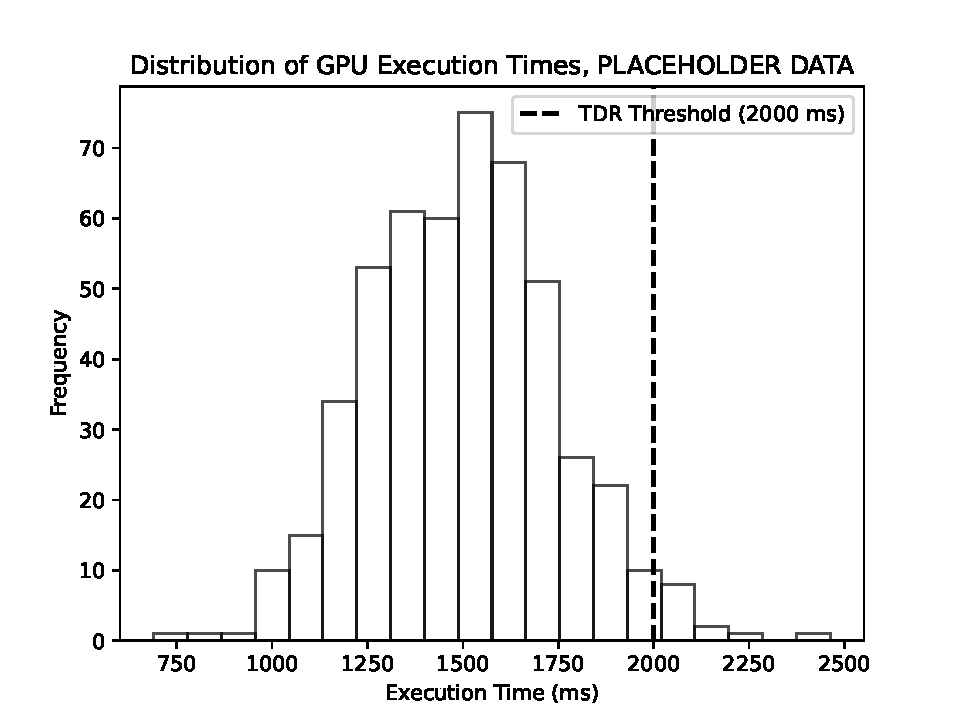
\includegraphics[width=\linewidth]{graphics/Figure_1.pdf}
  \caption{Execution times of \emph{Decoupled-Lookback (PLACEHOLDER DATA)}}
\end{figure}

Exacerbating this issue is the fact that no major graphics API currently provides developers with a mechanism to query FPG support. This lack of transparency forces developers to design algorithms without clear knowledge of whether critical guarantees are available on the target hardware. In environments like shading languages, where cross-platform portability is required, this uncertainty compels developers to revert to older, less efficient strategies such as \emph{Reduce-Then-Scan}. Yet, in the absence of guaranteed forward progress, developers have little choice but to sacrifice performance for broader compatibility.

\subsection{Earlier Attempts at Portability}
Levien and Naur~\cite{Raph2021} made the first attempt at implementing a \emph{DecoupledLookback} approach without forward progress requirements in \emph{ScalarFallback}. Each time a workgroup spins on a preceding tile, it advances a \emph{fallback} operation by incrementally consuming the blocking tile---one element at a time. By enabling workgroups to operate on data from other tiles, \emph{ScalarFallback} prevents deadlocking by targeting the \emph{mutual exclusion} condition described by Coffman et al. While this may involve performing redundant work when a tile is late rather than genuinely blocking, it ensures the algorithm's termination by allowing any workgroup to complete the reduction of a blocking tile, thereby breaking inter-workgroup dependencies.

\emph{ScalarFallback} suffers from two primary issues that impact its efficiency. First, the fallback reduction is performed serially by a single thread, progressing only when the workgroup engages in a waiting spin. This effectively takes $t$ spins to complete the fallback of a blocking $t$-sized tile. Moreover, because only a single thread is responsible for loading elements, the cache line associated with the loaded elements is severely underutilized, further degrading performance. Second, once the fallback is complete, the workgroup does not post its result to device memory. Consequently, every workgroup deadlocked by that tile must redundantly execute the fallback, wasting computational resources. While \emph{ScalarFallback} was able to achieve speed of light on hardware supporting FPG and executed correctly on hardware without FPG, its performance on the latter was inferior to that of \emph{Reduce-Then-Scan}.

\section{Decoupled-Fallback}
\thomas{I've broken somewhat with the outline and moved the goals and non-goals section to somewhere in the introduction. I kept finding myself trying to write around it. I think the content there is good, but it's very awkward as it ended up so deep within the paper. The placement of this section here feels more natural, and seems to mirror other papers?}
\emph{Decoupled-Fallback} separates fallback operations from the lookback process, enhancing the \emph{Scalar-Fallback} technique with significantly improved fallback performance. As an extension of the \emph{Chained-Scan} architecture, it retains the advantages of high speed and oversubscription, aligning with our design requirements.

\thomas{What I want to accomplish here is to go beyond saying "Here is our method. It works great." I want to show that these are the possible avenues to attack deadlocking . . . and exhaustively demonstrate that removing mutual exclusion is the best way to do it, under our given constraints.}
Like \emph{Scalar-Fallback}, we choose \emph{mutual exclusion} as our approach to break deadlocking. \emph{Dependency relationships} and \emph{no preemption} are immutable characteristics of scan and the GPU programming model, eliminating them as viable avenues for breaking deadlocking. While it may be possible to break \emph{circular ordering} by designing tile sizes such that workgroups are mapped one-to-one to multiprocessors, doing so portably is infeasible. Moreover, vendor guidance on progress guarantees among multiprocessors is also lacking, leaving the same risks of deadlocking but at the multiprocessor level. While eliminating \emph{resource holding}---allowing workgroups to discard work tiles when they encounter a deadlock---is theoretically possible, it is strictly worse than eliminating \emph{mutual exclusion}, as it necessitates $t$ additional movements (discard-read-read versus read).
\begin{algorithm}[htb]
  \small
  \SetAlgoLined
  \KwGlobalIn{%
    $in[]$,
    $out[]$,
    $spine[]$,
    $tileBump$,
  }
  \KwSharedIn{%
    $wg\_partials[]$,
    $wg\_fallback[]$,
    $wg\_prev\_reduction$,
    $wg\_broadcast$,
    $wg\_control$,
  }
  \KwGlobalOut{$out[]$ inclusive scan of $in[]$}
  \KwConstants{Vectors per thread $p$}

  \If{$threadid = 0$}{
    $wg\_broadcast \gets atomicAdd(\&tileBump, 1)$\;
    $wg\_control \gets LOCKED$\;
  }
  \textbf{barrier()}\;

  $part\_id \gets wg\_broadcast$\;

  \textit{local\_vectors}: $\textnormal{array}\langle \textnormal{vec4}\langle u32\rangle, p\rangle$\;

  \textbf{Load}($in$, $part\_id$, \textit{local\_vectors})\;
  \textbf{SubgroupRake}(\textit{local\_vectors})\;

  \If{$highestRankLane(threadid)$}{
    $wg\_partials[subgroup\_id] \gets local\_vectors[final\_partial]$\;
  }
  \textbf{barrier()}\;

  \textbf{WorkgroupWideScan}($wg\_partials$)\;
  \textbf{barrier()}\;

  \tcp{Decoupled Fallback}
  \While{$wg\_control = LOCKED$}{
    \textbf{Lookback}($spine$, $wg\_prev\_reduction$, $wg\_control$)\;
    \textbf{barrier()}\;

    \If{$wg\_control = LOCKED$}{
      \textbf{FallbackReduce}($in$, $wg\_fallback$)\;
      \textbf{FallbackInsertionAttempt}($spine$, $wg\_fallback$, $wg\_prev\_reduction$, $wg\_control$)\;
      \textbf{barrier()}\;
    }
  }

  \textbf{Write}($out$, $part\_id$, \textit{local\_vectors}, $wg\_partials$, $wg\_prev\_reduction$)\;

  \caption{High-Level Scan Kernel}
\end{algorithm}

To optimize the fallback operation, we employ three strategies. Although a lookback is performed by a single thread or subgroup, we want the entire workgroup to participate in the fallback. To achieve this, our first strategy is the use of a workgroup-wide \emph{control flag}, which enables threads performing the lookback to signal the entire workgroup when a fallback is necessary. Second, we explicitly limit the number of spins a workgroup can perform while waiting on a tile. If this maximum spin count is exceeded, the fallback operation is triggered. While this approach still risks performing redundant fallbacks---since a late tile is indistinguishable from one which is genuinely blocking---exposing the maximum spin count as a tunable parameter helps minimize false-positive fallbacks. Finally, after completing a fallback, the workgroup attempts to insert the reduction in place of the blocking tile, preventing subsequent workgroups from initiating redundant fallbacks.

The viability of \emph{Decoupled-Fallback} relies on the same cache locality properties as \emph{Decoupled-Lookback}. No subgroup scheduler is perfectly fair, and thus any given hardware will have a natural fallback rate $f$, regardless of FPG, due to \emph{false-positive} fallback operations. Consequently, we expect memory bandwidth traffic to increase (and throughput to decrease) by $O(fn)$ to $O((2 + f)n)$. However, just as serial ordering guarantees that memory accesses to the spine fall within an $o$-width sliding window, memory accesses to the scan input are similarly guaranteed to fall within an $ot$-width sliding window, making them also highly likely to reside within some level of the cache. As we later empirically demonstrate, this cache residency significantly reduces the cost of memory access, such that the fallback operation is almost always bound by the compute required to reduce the blocking tile. As a pure reduction incurs very lower overhead, we observe throughput approaching $O(2n)$ on most devices.

\section{Implementation}
At a high level, our algorithmn follows a five phase construction:
\begin{enumerate}
  \item[(0)] \textbf {Initialization}: The first thread in the workgroup atomically acquires its work-tile by atomically incrementing a value in global memory.
  \item \textbf{Load Phase}: Each thread loads $p$ vectors, consuming the input in a subgroup-blocked ordering. For a subgroup size $s$ and vector size $v$, each subgroup processes a contiguous block of size $s \cdot p \cdot v$.
  \item \textbf{Subgroup-Rake}: Each thread performs a private, serial scan across its vectors and then participates in $p$ raking subgroup scans. This allows the entire scan across the subgroup-block to be barrier-free and remain in registers. The final subgroup-block reduction is then posted to shared memory.
  \item \textbf{Workgroup-Wide Scan}: The workgroup collectively performs a scan across the subgroup partial reductions, writing the results back to shared memory upon completion.
  \item \textbf{Decoupled-Fallback}: The first subgroup in the workgroup performs a lookback operation, engaging in fallback operations if necessary. Once completed, it posts the results to shared memory for the workgroup to consume.
  \item \textbf{Write Phase}: Each subgroup incorporates the results from the workgroup-wide scan and lookback operation to produce and write out the correct output.
\end{enumerate}
Phase 0 ensures that the work tiles are consumed in serial order. Phases 1, 2, 3, and 5 comprise the intra-workgroup scan, following a \emph{Scan-then-Propagate} strategy. Phase 4, \emph{Decoupled-Fallback}, is responsible for managing all inter-workgroup dependencies.

\subsection{Intra-Workgroup Portability Adaptations}
As our loading and writing phase are typical of scan kernels, we focus here on our portability-specific adaptations.
\subsubsection{Subgroup-Raking}
We desire the smallest intra-workgroup spine possible. Not only does this reduce shared memory usage, but it also directly impacts the number of workgroup barriers encountered during the workgroup-wide scan, as this number is proportional to the size of the local spine. While large subgroups are relatively insensitive to this effect, small subgroups are particularly affected (reference depth here). To address this, we perform $p$ raking iterations of subgroup Kogge-Stone scans, where the highest-ranked thread passes its output into each succeeding scan. For a workgroup of size $w$, this approach reduces the number of partial reductions that each subgroup must post from $p$ to $1$, and it decreases the size of the spine from $\frac{pw}{s}$ to $\frac{w}{s}$.
\begin{algorithm}[htbp]
  \small
  \SetAlgoLined
  \KwSharedIn{ Array of subgroup partial reductions $x$ }
  \KwSharedOut{ Post-scanned array $x$ }
  \KwConstants{ Workgroup Size $W$, Subgroup Size $S$ }

  $spine\_length \gets W / S$\;
  $alignment \gets 1 << \text{divRoundUp}(\log_2(spine\_length), \log_2(S)) \cdot \log_2(S)$\;

  $stride \gets 1$\;
  $top\_offset \gets 0$\;

  \ForEach{$thread\_id$ \textbf{in} $W$ \textbf{in parallel}}{
    \For{$j \gets S$ \KwTo $alignment$ \textbf{with} $j \gets j \cdot S$}{
      \tcp{Brent-Kung Upsweep}

      $step \gets spine\_length / stride$\;

      \If{$thread\_id < step$}{
        $temp \gets \text{subgroupInclusiveScan}(x[thread\_id + top\_offset])$\;
        $x[thread\_id + top\_offset] \gets temp$\;
        \If{$\text{\normalfont highestRankLane}(thread\_id)$}{
          $x[(thread\_id / S) + step + top\_offset] \gets temp$\;
        }
      }

      \textbf{barrier()}\;

      \tcp{Fanout}

      \If{$j \neq S$}{
        $reduced\_stride \gets j / stride$\;
        $fanout\_index \gets thread\_id + reduced\_stride$\;

        $cond1 \gets fanout\_index < spine\_length$\;
        $cond2 \gets (fanout\_index \& (j - 1)) \geq reduced\_stride$\;

        \If{$cond1 \textbf{ \&\& } cond2$}{
          $x[fanout\_index] \gets x[fanout\_index] + x[((fanout\_index / stride) + top\_offset) - 1]$\;
        }
      }
      $stride \gets stride \cdot S$\;
      $top\_offset \gets top\_offset + step$\;
    }
    \textbf{barrier()}\;
  }
  \Return{$x$}\;
  \caption{Workgroup-Wide Scan. \john{Sorry to say that every one of those variable names need to be wrapped in \texttt{\textbackslash textit}. ``Typeset in math mode'' is not the same as ``Typeset in italics'' (see $offset$ vs.\ \textit{offset}).}}
  \label{alg:example}
\end{algorithm}

\subsubsection{Workgroup-Wide Scan}
The WebGPU specification supports subgroup sizes $s$, where $s = 2^k$ and $k \in [2, 7]$; on some hardware, subgroup sizes can vary between kernel launches. To handle this variability, we use a generalized radix-$s$ Ladner-Fischer~\cite{} scan network embedded with Kogge-Stone subgroup scans to perform the scan across the local spine. Because the upsweep phase of the Ladner-Fischer network follows a Brent-Kung~\cite{1675982} construction, assuming shared memory bank width equal to the subgroup size, any subgroup scans beyond the first will experience maximum $s$-way bank conflicts. To mitigate this, we employ a Merrill-Grimshaw~\cite[Section 3.3.5]{Merrill2009} style conflict avoidance strategy, which reduces bank conflicts to the radix base of the network—in our case, $s$. Counterintuitively, the resulting $s$-way conflict differs from the conflicts incurred by the Brent-Kung construction. Rather than multiple threads accessing different indices in the same memory bank, this conflict arises from a fanout originating from a single index. However, such access is interpreted by the hardware as a \emph{broadcast} operation, resulting in no conflicts. Although the Merrill-Grimshaw avoidance doubles our shared memory requirements, this increase is negligible due to our overall thriftiness, including the deliberate retention of vectors in registers and the efficiency of subgroup raking. Thus, this network offers several advantages: minimal depth of $\log_2 n$; asymptotically optimal $O(n)$ size; zero bank conflicts across all supported subgroup sizes.\footnote{Since we also require a workgroup-wide pure reduce operation, this can be achieved by omitting the fanout operation and substituting the subgroup Kogge-Stone scan with a subgroup butterfly reduction.}

\subsection{Decoupled-Fallback}
To reiterate, the goal of a lookback is twofold: to determine the reduction of all preceding work tiles and to communicate those values to succeeding tiles to accelerate their own lookback operations. Following the \emph{Decoupled-Lookback} technique, we model the spine as a finite state machine, where each work tile comprising the spine may exist in one of three states:
\begin{itemize}
  \item \textbf{Not Ready}: The tile has not yet been processed or written to global memory.
  \item \textbf{Ready}: The tile has completed its local reduction and posted it to global memory.
  \item \textbf{Inclusive}: The tile has completed its lookback and updated its posting to reflect the inclusive reduction.
\end{itemize}
Each lookback is, therefore, a traversal from the \emph{Ready} state to the \emph{Inclusive} state. To illustrate this process, we present a flowchart (SEE LOOKBACK FLOWCHART).
\john{It's helpful, I think, to also explicitly say what data is stored globally as the spine (I think, for each workgroup, one data element and one state).}

\subsubsection{Decoupled-Fallback}
\thomas{Given that "lock" has an extensive history of use in computer science and this is not that kind of lock, perhaps a better choice of phrase would be better. I've decided to refer to it as a "control flag"} \john{Good idea. ``Status flag'', perhaps?}
Prior to kernel launch, all tiles in the spine are initialized to the \emph{Not Ready} state. During partition index acquisition, we also initialize a shared memory \emph{control flag} to facilitate synchronization within the workgroup during the \emph{Decoupled-Fallback} phase. This flag governs both the initiation of fallback operations and the entry and exit of the entire phase, which begins immediately after the workgroup-wide scan over partial reductions is completed.
\john{Maybe a sentence that describes the state progression at a high level? e.g., ``the state of each workgroup begins at INVALID, moves to READY, then to INCLUSIVE, the state never moves backwards, each workgroup can operate independently and change its own state and also, during lookback, the state of preceding workgroups'', that sort of thing.}
\john{I might also say something like ``in the following discussion, we assume the `add' monoid and use terms like `add' and `sum', but the algorithm works with any monoid''. That gets rid of awkward terms like ``accumulate''. I don't feel strongly about this.}
\begin{figure}[h]
  \centering
  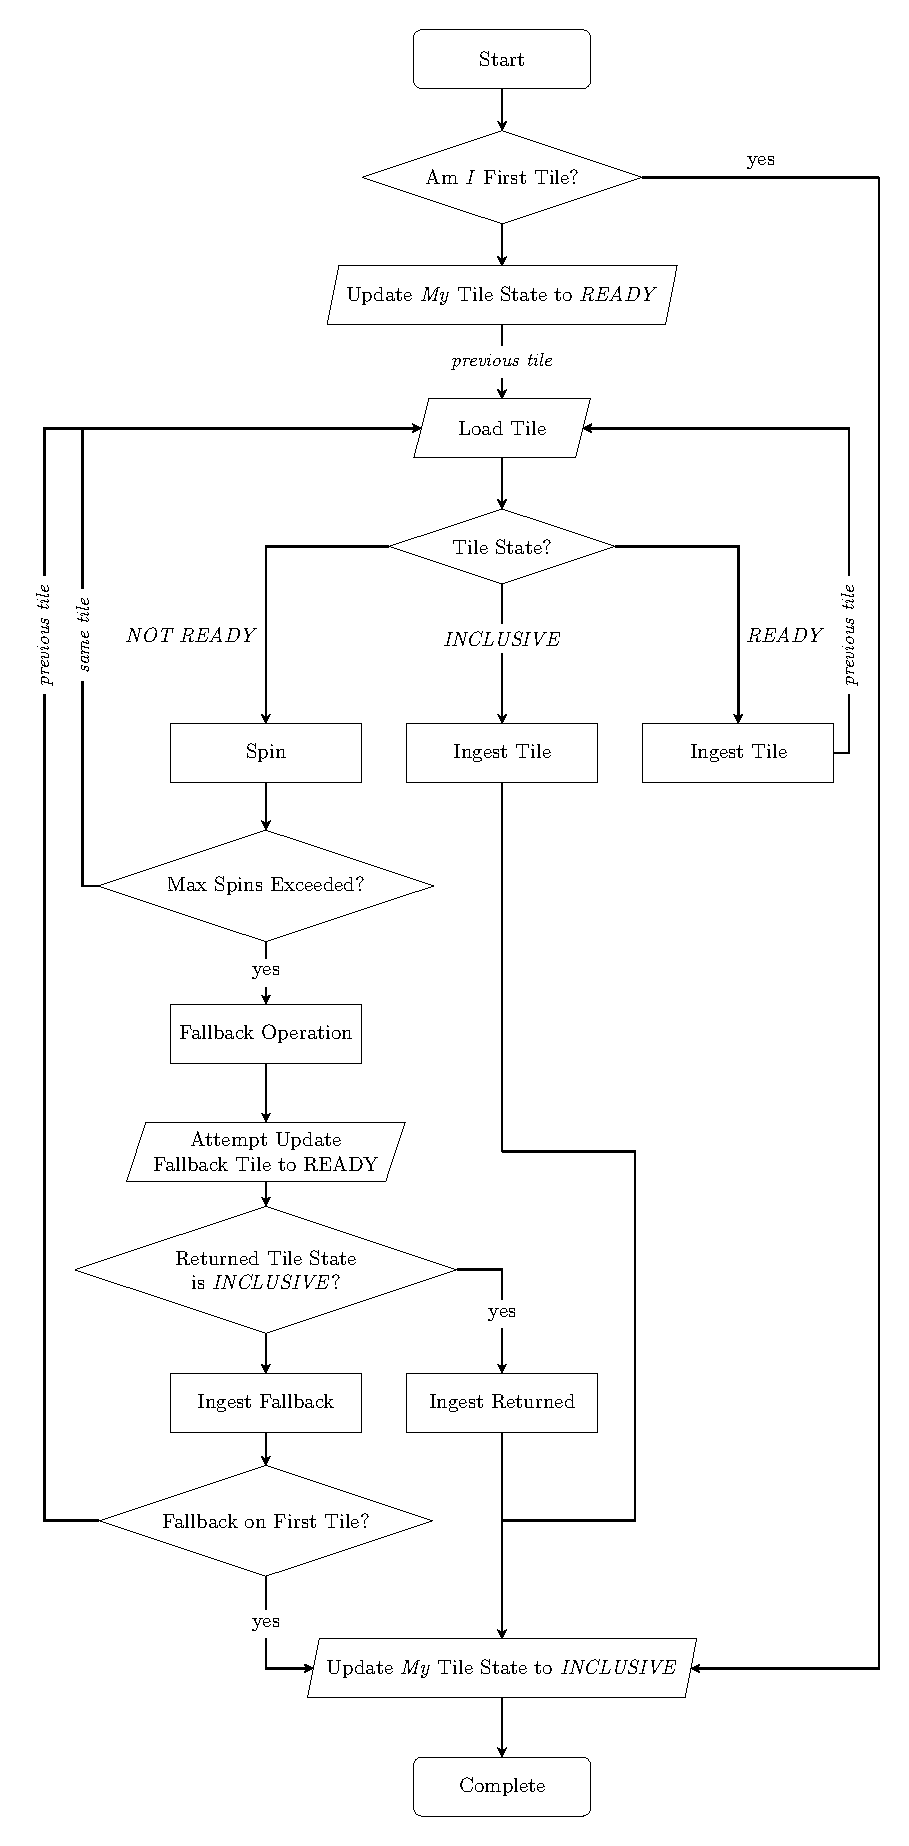
\includegraphics[width=\linewidth]{graphics/FlowChart.pdf}
  \caption{Decoupled-Fallback}
\end{figure}
\begin{enumerate}
  \item[(0)] \textbf{Posting Local Reduction:} Each workgroup posts its local reduction---the result of the workgroup-wide scan over partials---to global memory and updates its tile state to \emph{Ready}. If it is the first work tile, its local reduction \emph{is} its inclusive reduction. In this case, the workgroup updates its tile state directly to \emph{Inclusive} and bypasses the lookback entirely.

  \item \textbf{Initialization:}
        \begin{itemize}
          \item The control flag, initialized to \emph{Locked}, signals that the workgroup should enter the lookback phase.
          \item Each workgroup initializes a \john{shared workgroup-local (?)} \emph{previous reduction} variable with the identity element of the monoid to hold the accumulated reductions of preceding tiles.
          \item The workgroup prepares to traverse the spine, starting with its immediate predecessor tile. \john{Carefully look at the way this is worded with respect to ``immediate predecessor'' (previous sentence) vs.\ ``current'' (next sentence). I think here we want to say that we set the current tile to the immediate predecessor, and then the next sentence is consistent.}
        \end{itemize}

  \item \textbf{Lookback:}
        \begin{itemize}
          \item The workgroup queries the state of the current tile.
          \item If the tile is in the \emph{Ready} state, the workgroup accumulates the value and moves to \john{sets the current tile to} the preceding tile, repeating this step. \john{until reaching a tile that is not \emph{Ready}.}
          \item If the tile is in the \emph{Inclusive} state, the workgroup accumulates the value and proceeds directly to step 4.
          \item If the tile is in the \emph{Not Ready} state, the workgroup spins for a limited number of iterations, defined by the \emph{Maximum Spin Count}. If the spin count exceeds the \emph{Maximum Spin Count}, the workgroup signals a fallback operation \john{I don't get ``signals''. To whom are we signaling? What is signaled?} leaving the control flag \emph{Locked} and proceeds to the next step. \john{I think this is the place where decoupled-lookback fails without FPG\@. If so, say so, and why it fails. It underscores the central message of the paper, and is thus worth reiterating.}
        \end{itemize}

  \item \textbf{Fallback:} \john{Start with a sentence that describes \emph{why} we've reached this phase. ``Even after waiting, we see that a previous workgroup has not completed the reduction of its tile.'', that sort of thing.}
        \begin{itemize}
          \item The workgroup computes the reduction of the blocking tile by processing the corresponding elements directly. This process involves a workgroup-wide reduction using additional shared memory to aggregate partial subgroup results.
          \item Once the fallback reduction is complete, the workgroup \emph{attempts} to post the reduction to global memory and update the tile's state to \emph{Ready}.
          \item As this update attempt is performed atomically, the workgroup reads back the blocking tile's immediate state: \john{``immediate''? instead, ``most recent''?}
                \begin{itemize}
                  \item If the state is \emph{Inclusive}, the fallback value calculated by our workgroup is discarded, and our workgroup accumulates the value then proceeds to step 4.
                  \item If the blocking tile is the first in the spine, the workgroup has reached the start of the spine and proceeds to step 4.
                  \item Otherwise, the workgroup resumes the lookback, starting with the preceding tile. \john{\ldots\ by setting the current tile to \ldots\ I'm trying to not be sloppy with ``starting with'' given that we have a concept of ``current tile''.}
                \end{itemize}
        \end{itemize}

  \item \textbf{Finalization:}
        \begin{itemize}
          \item Upon completing the lookback or fallback, the local reduction is added to the \emph{previous reduction} to compute the inclusive reduction, which is then posted to global memory, transitioning the tile state to \emph{Inclusive}.
          \item The \emph{previous reduction} is posted to workgroup shared memory for the workgroup to consume and propagate as necessary. \john{``consume and propagate'' is super non-specific. What is happening here and how is it different than the next sentence?}
          \item The control flag is updated to \emph{Unlocked} to signal the exit of the \emph{Decoupled-Fallback} phase, allowing subsequent operations to proceed. \john{Be specific about what happens here! I'm presuming part of this item's work + the previous item's work is ``use the previous reduction as the starting point for scanning then outputting our current tile''. ``subsequent operations'' is super non-specific.} \john{In this item + the previous item, I bet there's some ordering constraints, either for correctness or for performance. For instance, I bet the highest priority is to add the previous reduction to my reduction and posting the result, since that propagation speed across tiles is probably really important for performance. Perhaps worth pointing out. Does the flag-unset have any ordering constraints in terms of correctness?}
        \end{itemize}
\end{enumerate}

\subsubsection{Tile State Implementation}
Because a tile may be in three possible states, two bits are required to record its state alongside the 32 bits needed to store the tile's reduction value. Previous \emph{Chained-Scan} architectures maintained a coherent view of both by using either 64-bit atomics with bit packing or memory fences with 32-bit atomics. However, neither approach is viable for our implementation, as WebGPU lacks a memory model and does not support 64-bit atomics. Additionally, 64-bit atomics are unsupported on most mobile devices, making their future adoption impractical for our needs. Instead, we use two 32-bit values, splitting the reduction into upper and lower 16-bit segments while reserving the two most significant bits of each 32-bit value to encode the tile state.
\begin{figure}[h!]
  \centering
  \includegraphics[width=\linewidth]{graphics/split.pdf}
\end{figure}
To accommodate the split values, we use a single subgroup for the lookback, leveraging subgroup \emph{ballot} to verify that the split value state is consistent across threads, and subgroup \emph{shuffle} to join and split reductions as needed. Since this method requires one thread per 16 bits, and the minimum subgroup size in the WebGPU specification is 4, it supports both 32-bit and 64-bit values. Notably, this extends support to 64-bit scans, which would not be possible even with 64-bit atomics.\footnote{Although native 64-bit values are not currently supported by the WebGPU specification, their future inclusion is anticipated.}

In the context of fallbacks, we require a tile state representation and an accompanying atomic operation that ensures a fallback update attempt can safely transition a tile's state to \emph{Ready} without overwriting a more advanced state. When an update attempt is made, the blocking tile can exist in any of the three states due to two scenarios: a false-positive fallback may have been initiated on a tile that transitions to \emph{Ready} or \emph{Inclusive} before the fallback completes, or another workgroup may have already successfully completed a fallback update, leaving the tile in \emph{Ready}. Consequently, the update mechanism should only overwrite tiles in the \emph{Not Ready} state. This requirement is further constrained by the fact that in WebGPU, the correctness of atomic \emph{Compare-and-Swap} is not guaranteed across all devices, prohibiting its use. To address this, we encode the tile state within the most significant bits of the split value and enforce a strict state ordering: \emph{Inclusive} $>$ \emph{Ready} $>$ \emph{Not Ready}. This design enables the use of atomic \emph{Maximum}, which inherently respects the state hierarchy, to safely perform updates.

\section{Evaluation}
\subsection{Experimental Setup}
We configure workgroups with a size of 256 threads, where each thread processes 4 vectors of size 4, resulting in 16 elements per thread and a total work tile size of 4096. We find a maximum spin count of 4 as offering good responsiveness to blocking, while minimizing false-positives fallbacks. As the size of the local spine is inversely proportional to the subgroup size, we allocate sufficient shared memory to accommodate the minimum subgroup size specified by the WebGPU standard, which is 4. Despite the additional shared memory required for conflict avoidance and fallback operations, total shared memory usage remains modest at only 1 KB. For all tests, we use an input size of $2^{25}$.

Something about devices here.
\subsection{Performance Comparison}
To evaluate the performance of \emph{Decoupled-Fallback}, we compare it against two key benchmarks: \emph{Reduce-Then-Scan} (RTS) and a \emph{Memcopy} operation. RTS serves as a baseline to demonstrate the performance gains of our approach over the previous FPG-constrained technique. Memcopy is included as a point of reference, as it shares the same $2n$ global memory movement required by scan operations.
\begin{figure}[h!]
  \centering
  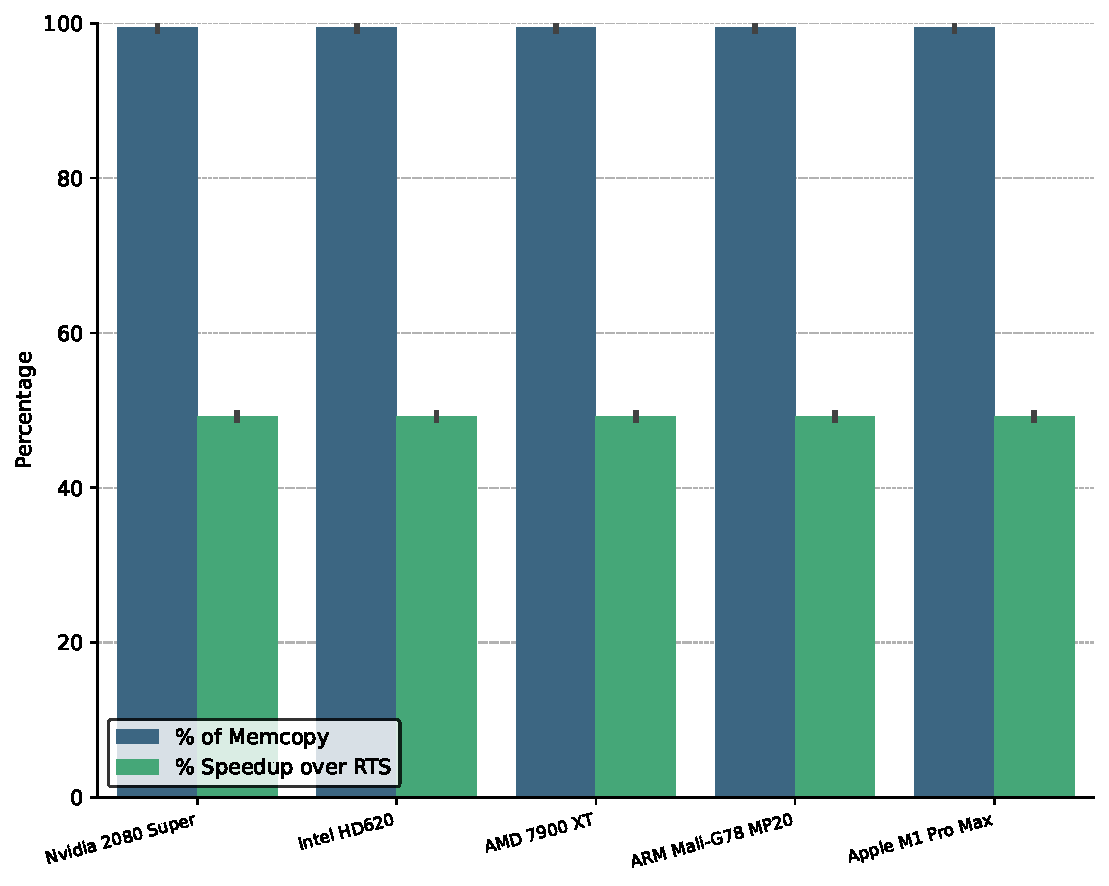
\includegraphics[width=\linewidth]{graphics/speedup.pdf}
  \john{\caption{This data (10 data points, which is pretty scant) is likely better presented as a table (also a better use of precious paper real estate). Also, make tables and figures float (don't do \texttt{[h!]}, just leave that blank, \LaTeX\ is good at page layout.)}}
\end{figure}
Since WebGPU limits device-side timestamps to compute or render passes, we implement a custom Memcopy kernel for timing purposes. Similarly, as there are no existing WebGPU implementations of RTS, we rely on our own optimized version for comparison. To ensure a competitive evaluation, our RTS implementation employs a variable-launch main kernel with a single workgroup performing a serial spine scan, as we found raking to be less performant in practice. Apart from this adjustment, the intraworkgroup implementation in RTS is identical to that used in \emph{Decoupled-Fallback}.

\thomas{Performance is good}

\subsection{How (un)fair is fair?}
Show the stats of each device. How many lookbacks?  How many fallbacks initiated? How many successful fallbacks?

\subsection{Simulated Blocking}
To demonstrate the resilience of our technique under fallback rates significantly higher than those observed organically on devices, we intentionally force fallbacks by omitting the posting of work tile reductions. Starting with infrequent omissions---1 in 512 workgroups---we progressively increase the rate to near-continuous levels, reaching 1 in 2 workgroups.
\begin{figure}[htbp]
  \centering
  \begin{subfigure}{.9\linewidth}
    \centering
    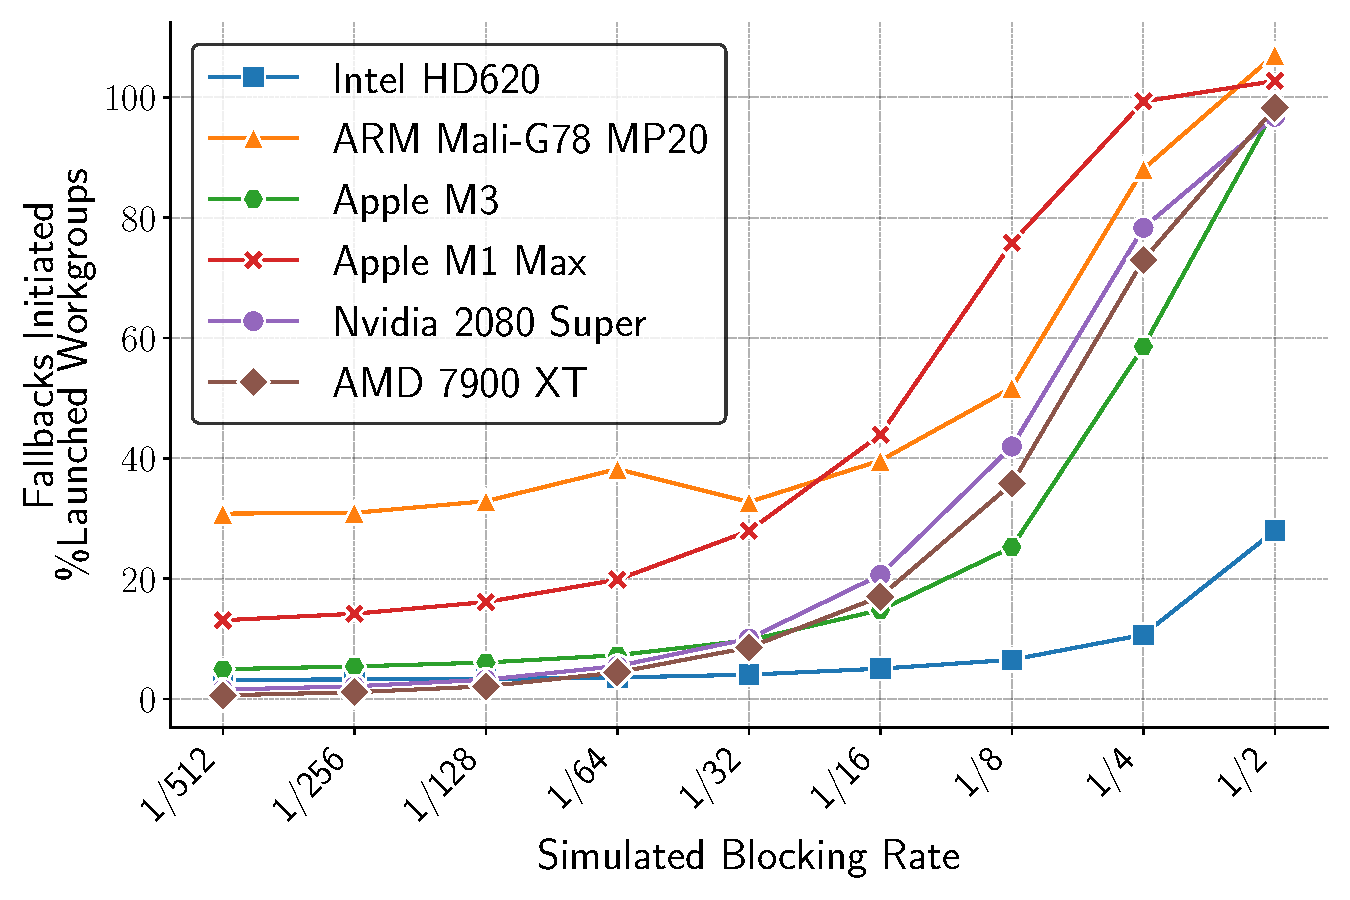
\includegraphics[width=\linewidth]{graphics/fallbacksInitiated_plot.pdf}
    \caption{Fallbacks Initiated}
    \label{fig:fallbacks_initiated}
  \end{subfigure}
  \begin{subfigure}{.9\linewidth}
    \centering
    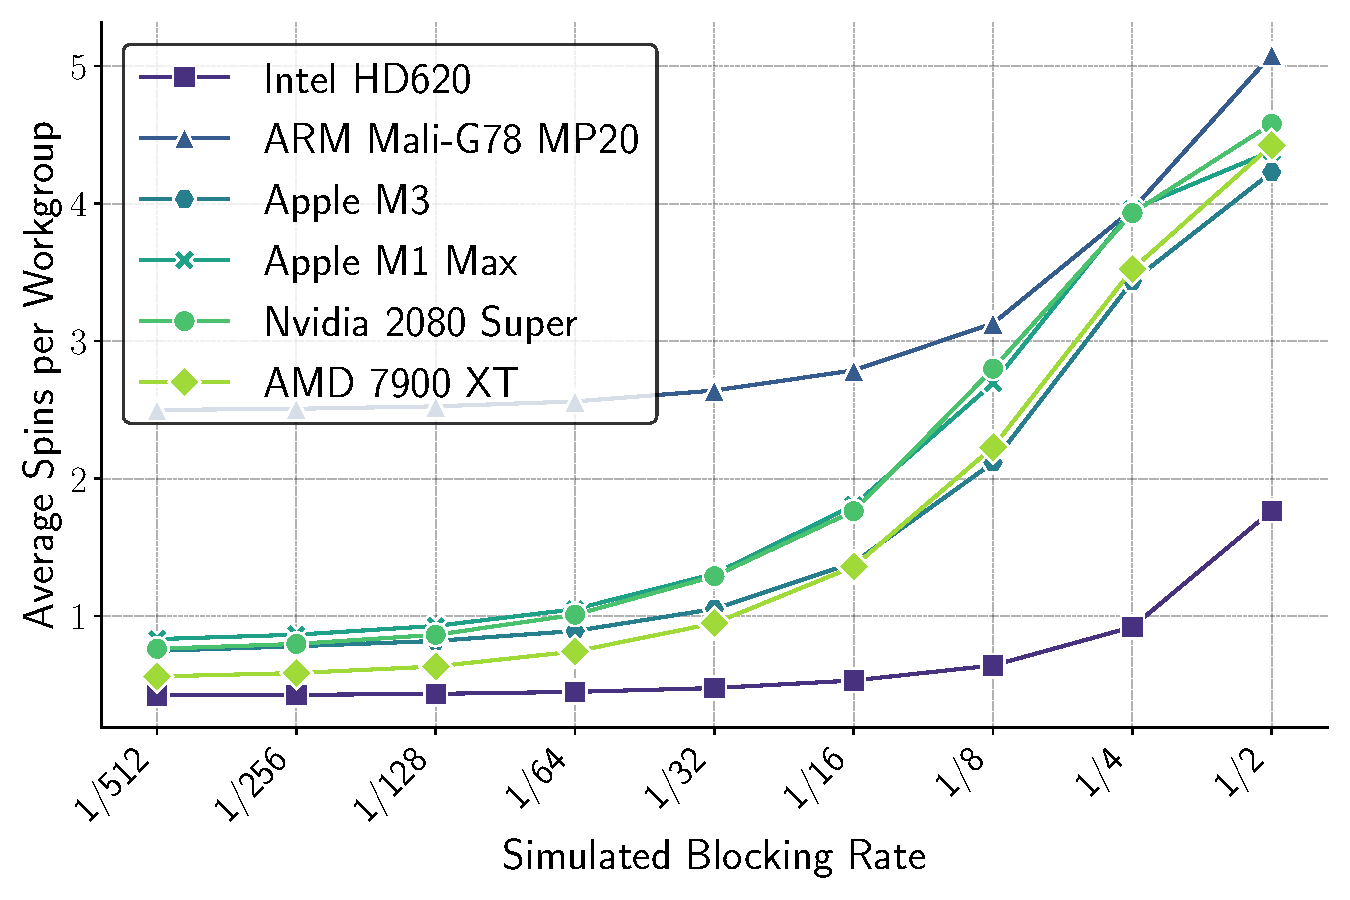
\includegraphics[width=\linewidth]{graphics/totalSpins_plot.pdf}
    \caption{Total Spins}
    \label{fig:total_spins}
  \end{subfigure}
  \begin{subfigure}{.9\linewidth}
    \centering
    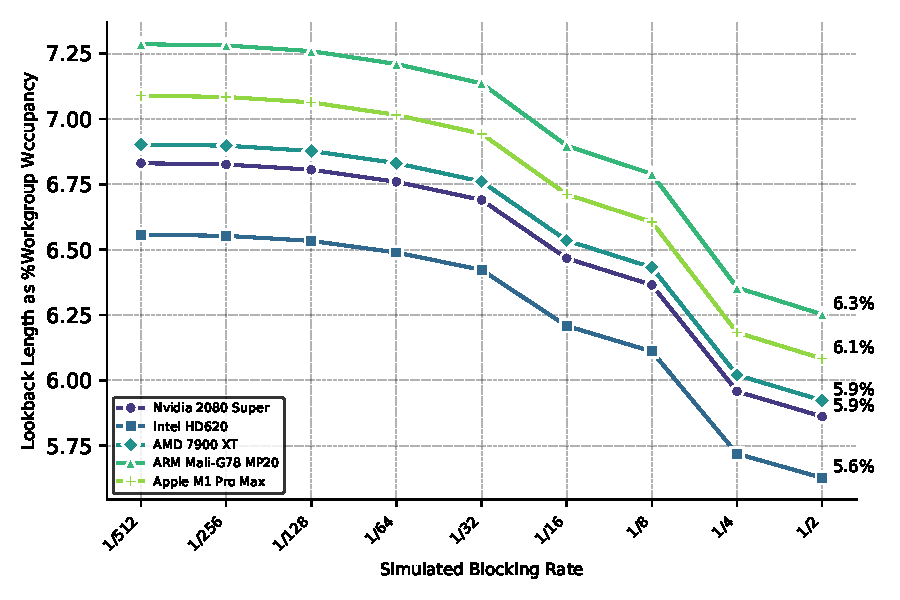
\includegraphics[width=\linewidth]{graphics/lookbackLength_plot.pdf}
    \caption{Lookback Length}
    \label{fig:lookback_length}
  \end{subfigure}
  \begin{subfigure}{.9\linewidth}
    \centering
    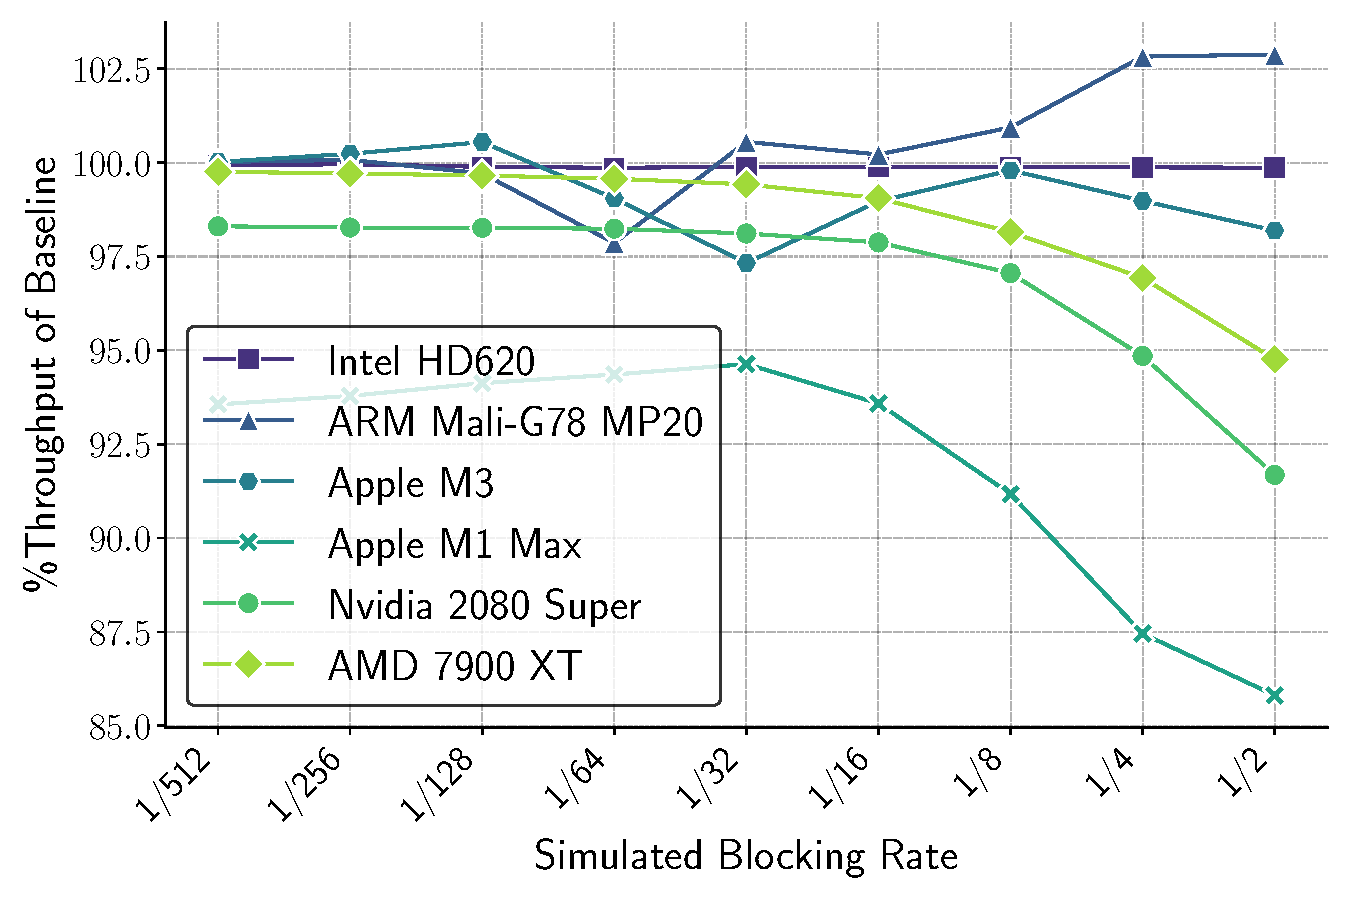
\includegraphics[width=\linewidth]{graphics/time_plot.pdf}
    \caption{Speed vs Memcopy}
    \label{fig:execution_time}
  \end{subfigure}
  \caption{Simulated Blocking}
  \label{fig:vertical_images}
\end{figure}

In Figure~\ref{fig:fallbacks_initiated}, we measure the number of fallbacks proportional to the number of workgroups launched, and verify that we are indeed inducing fallbacks. In Figure~\ref{fig:total_spins} we measure \thomas{this should be spins per workgroup it's a better metric}. In Figure~\ref{fig:lookbackLength} we see that. Finally, in Figure~\ref{fig:execution_time}, we can see that, even when \emph{half} the workgroups are deadlocking, \emph{Decoupled-Fallback} still achieves speeds of . . .

\section{Discussion}

\subsection{Trade-offs}

\subsection{Limits on Speed-of-Light Performance}
There are a number of factors which may preclude speed-of-light performance, but most salient is the fairness of the scheduling model. In \emph{Decoupled-Fallback}, a work tile which is late due to unfairness is indistinguishable from one which is blocking, so as a scheduler becomes increasingly unfair, it incurs an increasing number of redundant fallbacks. Consider a hardware with a workgroup occupancy denoted by $o$, and let $f$ represent the probability that a fallback operation occurs at a particular lookback step. Because the number of lookback steps is bounded by $o$, the expected number of fallback operations is approximately $fo$. This results in a factor of $fo$ increase in global memory reads and a factor of $fo\log{n}$ increase in work.

This increased sensitivity to fairness exacerbates existing issues which negatively impact the performance of previous scan architectures, namely lack of compute, and slow atomic update latency. On hardware that lacks sufficient compute power to be memory-bandwidth bound, the additional work incurred by redundant fallback reductions is particularly deleterious. High atomic update latency further compounds the problem: as inter-workgroup communication time grows, the minimum delay before updates become visible to dependent workgroups also increases. This, in turn, raises the number of lookback steps that may be needed and potentially leads to redundant fallbacks.

\thomas{Somewhere in here is perfect for Raph's commentary on the speed of atomics on different hardware. Once we have it, we can retool this section around it.}

\section{Cut material, can be readded if we have enough space}

To ensure consistency with our coding artifact and promote cross-vendor compatibility, we use the terminology of the WebGPU specification.
\setlength{\tabcolsep}{3pt}
\begin{table}[h]
  \centering
  \caption{Non-Exhaustive Equivalent Terminology}
  \label{tab:terminology}
  \begin{tabular}{lcccc}
    \toprule
    \textbf{WGSL} & \textbf{GLSL} & \textbf{HLSL} & \textbf{Metal} & \textbf{CUDA} \\ \midrule
    Subgroup      & Subgroup      & Wave          & SIMD-group     & Warp          \\
    Workgroup     & Workgroup     & Group         & Threadgroup    & Block         \\
    Workgroup     & Shared        & Groupshared   & Threadgroup    & Shared        \\ \bottomrule
  \end{tabular}
\end{table}

Despite its limited suitability within the oversubscription paradigm, inter-workgroup synchronization holds significant performance potential, as many GPU-friendly algorithms—such as \emph{example}, \emph{example}, and \emph{scan}---can benefit from a trade-off that eliminates the costly overhead of kernel-launch synchronization. This potential was explored in prior work~\cite{}, culminating in Gupta et al.’s~\cite{} \emph{Persistent Thread} paradigm. Rather than oversubscribing processors by launching $b$ workgroups, each consuming a single \emph{work tile}, this approach \emph{discovers} the total workgroup occupancy across the device $o$---referred to by Gupta et al. as a \emph{maximal launch}---and launches $o$ workgroups, each responsible for processing $b/o$ work tiles. Limiting the launch size allows the workgroups to always remain on chip, eliding context switching, and thus facilitating an efficient inter-workgroup barrier.

\subsection{Work Efficiency and Depth}
\subsubsection{Size Agnostic Scan}
For a subgroup of size $s$, the Kogge-Stone network has a work complexity of $s \log_2 s$. Given an input of size $n$, the work complexity is:
\begin{equation}
  \begin{aligned}[b]
    \text{Work} & = \underbrace{\vphantom{\sum_{k=0}^{\lceil \log_s n \rceil}}n}_{\text{fanout}}
    +
    \underbrace{\sum_{k=1}^{\lceil \log_s n \rceil}}_{\text{iterations}}
    \underbrace{\vphantom{\sum_{k=1}^{\lceil \log_s n \rceil}}\frac{n}{s^k}}_{\text{calls per iteration}}
    \cdot
    \underbrace{\vphantom{\sum_{k=1}^{\lceil \log_s n \rceil}}s \log_2 s}_{\text{work per call}} \\
                & = n + s \log_2 s \cdot \sum_{k=1}^{\lceil \log_s n \rceil} \frac{n}{s^k}       \\
                & = O\left(n + n \log_2 s\right)                                                 \\
                & = O(n \log_2 s).
  \end{aligned}
\end{equation}
Since the subgroup size remains constant within each kernel launch, the final work complexity is $O(n)$. Thus our implementation preserves asymptotically optimal work, even though the structure is not isomorphic to the radix-two network. The Kogge-Stone scan has a depth of $\log_2 s$ Thus, the total depth of the scan is:
\begin{equation}
  \begin{aligned}[b]
    \text{Depth} & = \underbrace{\lceil \log_s n \rceil}_{\text{loop iterations}}
    \cdot \underbrace{\log_2 s}_{\text{depth per iteration}}                           \\
                 & = \left\lceil \frac{\log_2 n}{\log_2 s} \right\rceil \cdot \log_2 s \\
                 & = \log_2 n + O(1).
  \end{aligned}
\end{equation}
While minimal depth is preserved regardless of the subgroup size, this result can be somewhat misleading, as the depth incurred during the subgroup portion of the scan requires no barrier, whereas the main loop incurs a workgroup-wide barrier at each iteration. Consequently, while the theoretical depth remains constant across subgroup sizes, smaller subgroups tend to perform worse in practice due to the increased relative cost of synchronization and the overhead of additional iterations in the main loop.
\begin{acks}
\end{acks}

\bibliographystyle{ACM-Reference-Format}
\bibliography{bib}

\appendix
\section{Artifact}

\subsection{Availability}
We provide our artifact in the following GitHub repository:
\thomas{Will anonymize with GithubAnonymous once we are ready.}
Due to the aforementioned issues with WGSL transpilers, we choose Dawn as our WebGPU implementation.

\subsection{Requirements}

\subsubsection{Device Requirements}
Any device supporting Dawn, with subgroup and timestamp query capabilities, and at least 384 MB of available device memory.

\subsubsection{Software Requirements}
\begin{itemize}
  \item Git
  \item CMake 3.10.2+ or another C++ build tool
  \item C++17-compliant compiler
  \item Python for fetching dependencies
\end{itemize}

\subsection{Building}
Although native WebGPU is supported on various operating systems—most notably Windows, macOS, and Linux—this section will focus on building it in Unix-like environments for the sake of brevity, using CMake as the example build tool.

\subsubsection{Building Dawn}
\begin{enumerate}
  \item[(0)] Dawn depends on the following packages (Ubuntu package names):
        \begin{lstlisting}[basicstyle=\ttfamily\small, frame=single]
sudo apt install libxrandr-dev
  libxinerama-dev libxcursor-dev libxi-dev \
  libx11-xcb-dev mesa-common-dev
  \end{lstlisting}

  \item Clone the Dawn repository:
        \begin{lstlisting}[basicstyle=\ttfamily\small, frame=single]
git clone https://dawn.googlesource.com/dawn
RESET HEAD here to a specific commit. . . to lock in?
  \end{lstlisting}

  \item Build and install Dawn with your build tool and compiler of choice:
        \begin{lstlisting}[basicstyle=\ttfamily\small, frame=single]
cd dawn
cmake -S . -B out/Release \
  -DDAWN_FETCH_DEPENDENCIES=ON \
  -DDAWN_ENABLE_INSTALL=ON \
  -DCMAKE_BUILD_TYPE=Release
...
cmake --build out/Release
...
cmake --install out/Release \
  --prefix install/Release
  \end{lstlisting}
\end{enumerate}

\subsubsection{Building Artifact}
After successfully building and installing Dawn, follow these steps to build the artifact:

\begin{enumerate}
  \item Navigate to the artifact directory:
        \begin{lstlisting}[basicstyle=\ttfamily\small, frame=single]
cd Decoupled-Fallback-Paper/artifact/Dawn
  \end{lstlisting}

  \item Set the `CMAKE\_PREFIX\_PATH` to point to your Dawn installation directory:
        \begin{lstlisting}[basicstyle=\ttfamily\small, frame=single]
export CMAKE_PREFIX_PATH=/path/to/ \
dawn/install/Release
  \end{lstlisting}

  \item Build the artifact:
        \begin{lstlisting}[basicstyle=\ttfamily\small, frame=single]
cmake -S . -B out/Release \
  -DCMAKE_BUILD_TYPE=Release
  \end{lstlisting}

  \item Compile the project:
        \begin{lstlisting}[basicstyle=\ttfamily\small, frame=single]
cmake --build out/Release
  \end{lstlisting}
\end{enumerate}



\end{document}
\endinput

%%% Local Variables:
%%% mode: LaTeX
%%% TeX-master: t
%%% End:
